\documentclass[../main.tex]{subfiles}

% Opis baze podataka

\begin{document}
U ovom poglavlju će biti opisan modela baze podataka koji je predstaljen pomoću ER dijagrama \textit{(eng.} entity-relationship diagram\textit{)} prikazanog na slici\footnote{Za bolji prikaz slike pogledati \href{https://github.com/jovanape/Informacioni-sistem-za-teretane/blob/main/Dijagrami/jpg_fajlovi/EER\%20dijagram\%20baze\%20podataka\%20-\%20novo\%202.jpg}{ovde.} } \ref{fig:baza} . Svi entiteti koji se pojavljuju prate opise slučajeva upotrebe iz prethodnog poglavlja. Pojedini entiteti su specifični samo za pojedinačne slučajeve upotrebe, dok su entiteti kao što su \textit{Trening} i \textit{Klijent} zastupljeni u većini slučajeva. 


\begin{figure}[!ht]
\begin{center}
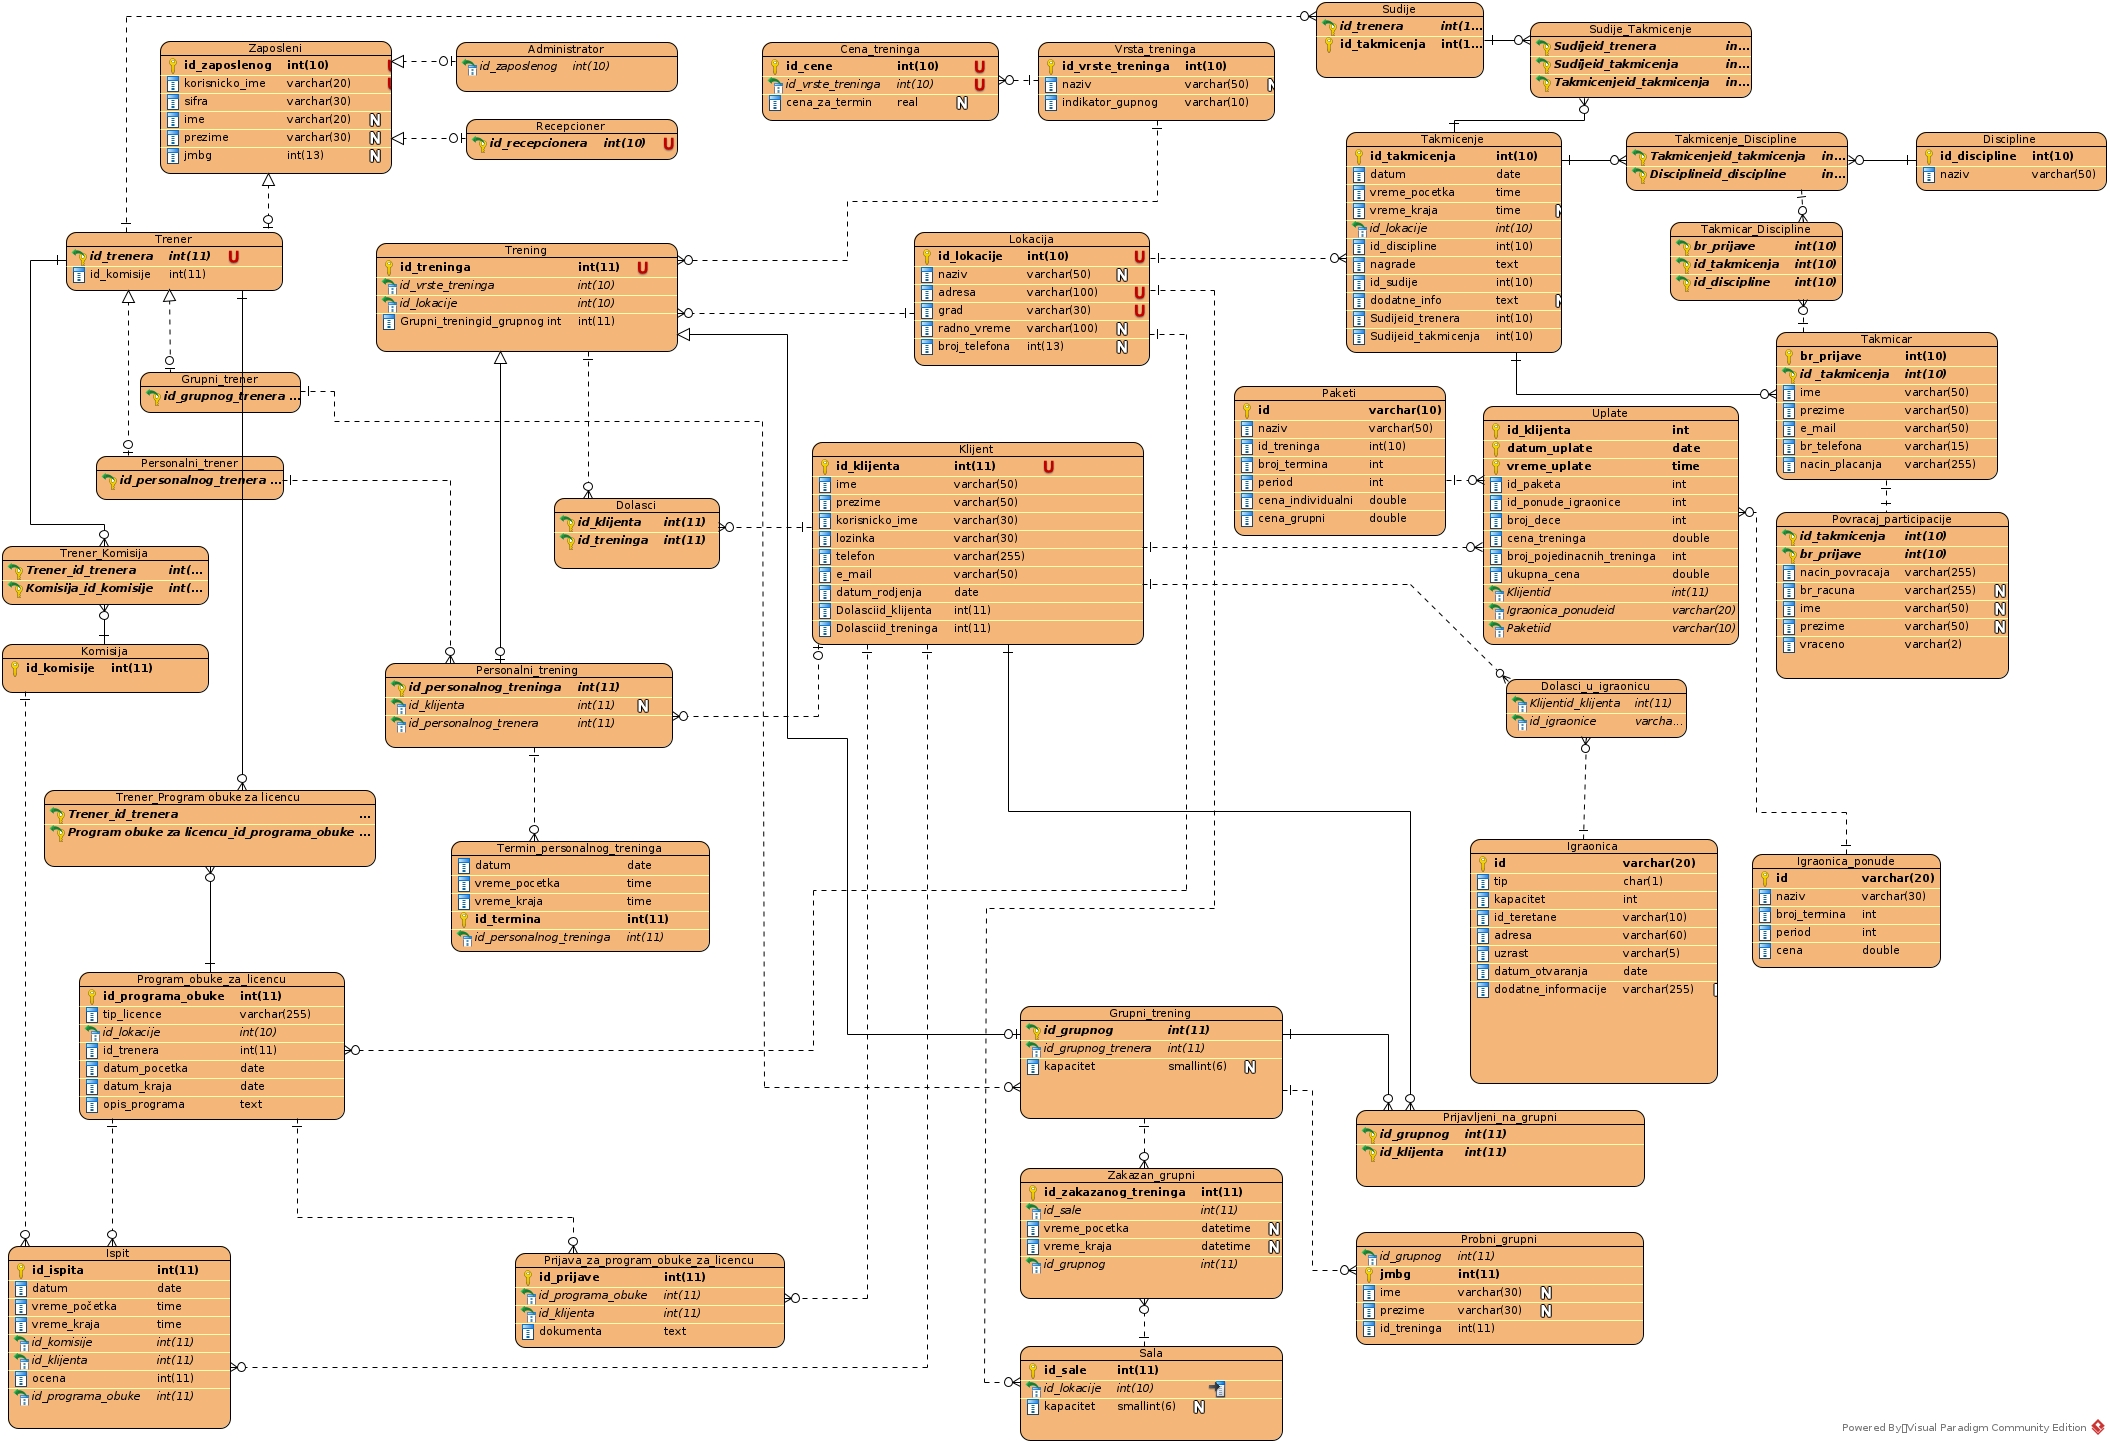
\includegraphics[scale=0.20]{sections/images/EER dijagram baze podataka - novo 2.jpg}
\end{center}
\caption{ER dijagram baze podataka}
\label{fig:baza}
\end{figure}

\subsection{Opis entiteta}


\subsubsection{Entitet Zaposleni}

Entitet \textit{Zaposleni} čuva osnovne podatke o zaposlenima. Njegovu hijerahiju čine svi tipovi zaposlenog: \textit{Administrator}, \textit{Trener} i \textit{Recepcionar}. A \textit{Trener} predstavlja generalizaciju za entitete \textit{Personalni trener} i \textit{Grupni trener}


\subsubsection{Entitet Klijent}
U entitetu \textit{Klijent} se čuvaju sve lične informacije za svakog klijenta. Takođe u ovom entitetu se vodi evidencija dolazaka klijenta na treninge. Atributi ovog entiteta su: id\_klijenta, ime, prezime, korisnicko\_ime, lozinka, telefon, e\_mail, datum\_rodjenja, Dolasciid\_klijenta i  Dolasciid\_treninga.
% PREDLOG: Nazvati poslednja 2 atributa dolasci_id_klijenta, dolasci_id_treninga - samo ispraviti ER model. U tom slucaju, promeniti i ovde te nazive.
Atribut id\_klijenta predstavlja njegov jedinstveni broj, na osnovu koga se on identifikuje. U nekim delovima projekta ovaj broj id\_klijenta se naziva i članska karta. 
Entitet \textit{Klijent} je povezan sa entitetom \textit{Uplate}, tako da jedan klijent može da izvrši više uplata, ali jedna uplata ne može biti izvršena od strane više klijenata. Zatim, entitet \textit{Klijent} je povezan sa entitetom \textit{Dolasci\_u\_igraonicu}, tako da u jednu igraonicu može biti više klijenata, ali jedan klijent ne može istovremeno biti u više igraonica. %Dalje, entitet Klijent je povezan sa entitetom Grupni\_trening, tako da više klijenta mogu biti na jednom istom grupnom treningu, ali ne može jedan klijent istovremeno da bude na više različitih grupnih treninga. % Klijent (vise) nije povezan sa Grupni\_trening
Dalje, entitet Klijent je povezan sa entitetom Prijavljen\_na\_grupni pomoću kog se vodi evidencija o prijavljenim klijentima na grupne treninge. Jedan klijent može biti prijavljen na više grupnih treninga.
\textit{Klijent} je povezan i sa entitetom \textit{Personalni trening}, o kom će biti više reči u nastavku.
Pomoću agregiranog entiteta \textit{Dolasci} vodi se evidencija o dolasku klijenata na treninge.
% Igraonice - klijenti?
% Igraonice - deca?
% Korisnik nije opisan do kraja, treba ga povezati sa preostalim entitetima, tj. opisati te veze.


\subsubsection{Entitet Lokacija}

\textit{Lokacija} predstavlja lokaciju i osnovne podatke o konkretnoj teretani iz lanca, kao što su naziv, adresa, grad, radno vreme i broj telefona.
Entite \textit{Lokacija} sa entitetom \textit{Sala} ima One to Many relaciju predstavljena stranim ključem id\_sale. 


\subsubsection{Entitet Paketi}
Entitet Paketi sadrži podatke koji su neophodni za formiranje različitih ponuda koje ova teretana nudi korisnicima. Svaki paket ima svoj jedinstveni identifikator - to je atribut id. Zatim, ima i atribute: naziv, id\_treninga, broj termina, period - koji predstavlja vreme trajanja (tj. vreme važenja tog paketa), cena\_individualni - koji predstavlja cenu za individualni trening, cena\_grupni - koji predstavlja cenu za grupni trening. Kada klijent odabere paket koji mu, po svim ovim informacijama odgovara, uplaćuje novac, i to se evidentira u entitet Uplate (opisan u nastavku). Jedan isti paket može da bude prisutan u više uplata. Obrnuto nije moguće.


\subsubsection{Entitet Uplate}

Entitet uplate sadrži informacije o svim uplatama koje su uspešno izvršene. Atributi ovog entiteta su: id\_klijenta, datum\_uplate, vreme\_uplate, id\_paketa, id\_ponude\_igraonice, broj\_dece, cena\_treninga, broj\_pojedinacnih\_treninga, ukupna\_cena, Klijentid, Igraonica\_ponudeid, Paketiid.
% PREDLOG: Nazvati poslednja 3 atributa malim slovima i "_". Onda, promeniti i ovde te nazive.
Entitet Uplate povezan je sa entitetom Klijent, jer je klijenti ti čije se uplate čuvaju u ovom entitetu. I to, jedan klijent može da ima više uplata. Jedna uplata ne može imati više klijenta. Takođe, entitet Uplate je povezan i sa entitetom Paketi, gde jedan paket može da bude uplaćen više puta (na primer, dva različita korisnika mogu da uplate isti paket), ali jedna uplata ne može da sadrži više od jednog paketa (a ni manje, osim ako je neko uplatio igraonicu). Entitet Uplate povezan je još sa entitetom Igraonica\_ponude, i to tako da jedna jedna ponuda igraonice može javiti u jednoj uplati (ili ni jedna, ako je neko uplatio paket). S druge strane, ne mogu više ponuda igraonice da se nađu u jednoj istoj uplati.


\subsubsection{Entitet Igraonica}
Igraonice predstavljaju dodatni sadržaj teretana koje pripadaju ovom sistemu teretana. Najveći značaj ovih igraonica imaju roditelji sa (malom) decom, jer dok oni treniraju, njihova deca mogu ovde da borave. Postoje dva tipa igraonica, a to su, dečija igraonica i PS (eng. PlayStation, PS) igraonica. Svaka od njih ima uslove koje treba ispoštovati. Na primer, u dečiju igraonicu mogu da dolaze samo deca mlađeg uzrasta, dok u PS igraonicu ne mogu da dolaze deca ispod određenog uzrasta. Takođe, svaka igraonica ima ograničen kapacitet, koji se ne sme prekoračiti. Osim toga, bitno je kada je igraonica otvorena, gde, i u sklopu koje teretane.
% Svaka teretana može imati najviše jednu dečiju igraonicu i najviše jednu PS igraonicu.
U bazi, unutar entiteta Igraonica, čuvaju se vrednosti sledećih atributa: id, tip, kapacitet, id\_teretane (kojoj ta igraonica pripada), adresa, uzrast, datum\_otvaranja, dodatne\_informacije. Atribut dodatne\_informacije može i ne mora da sadrži neke dodatne podatke, kao što su broj PS uređaja u PS igraonici, i drugo. Entitet Igraonica je povezan sa entitetom Dolasci\_u\_igraonicu, jer je negde potrebno voditi evidenciju o dolascima. Jedna igraonica se može javiti više puta unutar entiteta Dolasci\_u\_igraonicu, ali ne može neko da bude istovremeno u više igraonica, te u jednom redu entiteta Dolasci\_u\_igraonicu ne može da se nađe više od jedne igraonice.


\subsubsection{Entitet Igraonica\_ponude}
Entitet Igraonica\_ponude je sličan entitetu Paketi, s tim što se ovde, na osnovu podataka iz ovog entiteta, formiraju ponude za igraonicu. Svaka ponuda ima svoj jedinstveni broj, odnosno identifikator, period važenja i broj termina koji ulazi u cenu te ponude. Atributi ovog entiteta su: id, naziv, broj\_termina, period i cena. Ovaj entitet je povezan sa entitetom Uplate. Naime, kada korisnik odabere ponudu za igraonicu i uspešno izvrši plaćanje, to se beleži u entitetu Uplate, u kome se beleže i sva druga plaćanja.


\subsubsection{Entitet Trening}

Entitet \textit{Trening} pomoću spoljašnjih ključeva id\_vrste\_treninga i id\_lokacije čuva informacije o vrsti treninga i lokaciji na kojoj se trening održava. \textit{Trening} se specijalizuje u entitete \textit{Personalni trening} i \textit{Grupni trening}.


\subsubsection{Entitet Sala}

\textit{Sala} predstavlja salu koja je odredjena lokacijom teretane i maksimalnim kapacitetom (maksimalan broj ljudi koji mogu trenirati u sali. Izmedju entiteta  \textit{Zakazan Grupni Trening} i sale postoji relacija Many to One. Prema tome postoji strani ključ id\_sale koji označava da povezuje salu sa grupnim treninzima koji se u njoj odvijaju. 

\subsubsection{Entitet Grupni trening}
\textit{Grupni trening} je vrsta entita \textit{Trening} koji održava \textit{Trener} grupi \textit{Klijenata}. Opisuje ga id\_treninga, id\_trenera i maksimalni kapacitet grupnog treninga.

\subsubsection{Entitet Zakazani grupni} je entitet koji će sadržati informacije o svim zakazanimm grupnim treninzima. Kao i kod \textit{Treninga} ima informacije o vremenu (početku i kraju treninga), id\_sale i id\_grupnog. Između entiteta \textit{Grupni trening} i \textit{Zakazani Grupni Treninga} postoji relacija One to Many predstavljena spoljnim ključem id\_grupnog.

\subsubsection{Entitet Prijavljeni grupni} 
Entit \textit{Prijavljeni grupni} čuva informacije o kandidatima i njihovim prijavljenim grupni treninzima. Između entiteta \textit{Grupni trening} i \textit{Prijavljeni grupni} postoji relacija One to Many predstavljena spoljnim ključem id\_grupnog. Dok između entiteta \textit{Klijent} i \textit{Prijavljeni grupni} postoji relacija One to Many predstavljena spoljnim ključem id\_klijenta.


\subsubsection{Entitet Probni trening} 
Entitet \textit{Probni trening} opisuje korisnike grupnih treninga koji prvi put prisustvuju i nisu registrovani korisnici. Zbog daljih provera, čuva se: JMBG, ime i prezime korisnika. Između entiteta \textit{Grupni trening} i \textit{Probni grupni} postoji relacija One to Many predstavljena spoljnim ključem id\_grupnog.

\subsubsection{Entitet Personalni trening}

Entitet \textit{Personalni trening} pomoću stranog ključa id\_personalnog\_trenera  čuva informaciju o tome koji trener drži dati trening, a pomoću stranog ključa id\_klijenta informaciju o tome koji klijent je prijavljen na dati trening. Ukoliko ni jedan klijent nije prijavljen, polje id\_klijenta ću biti null. Dodatno, \textit{Personalni trening} je povezan sa entitetom \textit{Termin personalnog treninga} koji sadrži informacije o datumu i vremenu početka i kraja treninga. 


\subsubsection{Entiteti vezani za Takmičenja}

Za grupu slučajeva upotrebe za takmičenja centralni entitet je \textit{Takmičenje}. On kao atribute ima jedinstveni identifikator koji čini primarni ključ, informacije o datumu, vremenu početka, vremenu kraja, dodatnim informacijama i nagradama i lokaciji. Informacije o disciplinama se dobijaju pomoću veze sa entitetom \textit{Discipline} koji čuva sve moguće discipline. S obzirom da na jednom takmičenju može biti više sudija, a sudije čine treneri teretane, kreiran je poseban entitet \textit{Sudije} koji čuva za svako takmičenje ko je sudija, a detaljnije informacije o osobama se mogu dobiti na osnovu veze sa entitetom \textit{Trener}. \textit{Takmičar} je poseban entitet koji se kreira pri registraciji novog takmičara i sadrži osnovne informacije koje se uzimaju popunjavanjem formulara.Njega jedinstveno određuje kombinacija broja prijave i id takmičenja. Takođe, povezan je vezom više-više sa \textit{Takmičenje\_discipline} koji predstavlja skup disciplina na koje je moguće prijaviti se za neko takmičenje. U slučaju da se takmičenje otkaže kreira se entitet \textit{Povracaj\_participacije} koji za svakog takmičara sa datog takmičenja čuva informacije na koji način mu vratiti novac i informaciju da li je vraćen - koja je inicijalno ne. 


\subsubsection{Entiteti vezani za Licencu}
Što se tiče obuke za licencu, centralni entitet te grupe slučajeva je \textit{Program obuke za licencu}. On sadrži informacije o tipu licence koja se dobija, lokaciji na kojoj se program održava, datumu početka i datumu kraja programa, kao i o tome koji treneri će držati obuku. Veza između \textit{Programa obuke za licencu} i \textit{Trenera} je više-više, pošto jednu obuku može da drži više trenera, a jedan trener može da drži više različitih obuka. \textit{Ispit} sadrži informacije o datumu, vremenu početka i kraja završnog ispita, klijentu koji polaže ispit, njegovoj oceni, kao i o komisiji koja je dala tu ocenu. Komisiju čini više trenera, a jedan trener može da bude član više komisija, pa je zbog toga između entiteta \textit{Komisija} i \textit{Trener} uspostavljena veza više-više. Evidencija o prijavama za obuku vodi se u agregiranom entitetu \textit{Prijava za program obuke za licencu} koji sadrži i dokumenta koja klijent mora da preda kako bi mogao da pohađa obuku.


\end{document}
